\documentclass[11pt]{scrartcl}
\usepackage[utf8]{inputenc}
\usepackage[croatian]{babel}
\usepackage{datetime}
\newdate{date}{14}{05}{2024}
\date{\displaydate{date}}
\usepackage[a4paper,margin=1in]{geometry}
\usepackage{amsfonts}
\usepackage{amsmath}
\usepackage{amssymb}
\usepackage{amsthm}
\usepackage{csquotes}
\usepackage{tcolorbox}
\usepackage{tikz}
\usepackage{arydshln}
\pagenumbering{gobble}
\usepackage{float}
\usepackage{xcolor}
%\usepackage[dvipsnames]{xcolor}
%\usepackage{mathptmx} %times new roman?
\usepackage{breqn}
\usepackage[T1]{fontenc}
\usepackage{thmtools}
\usepackage{multirow}
\usepackage[unicode]{hyperref}

\usepackage{booktabs}
\usepackage{listings}

\definecolor{seagreen}{HTML}{21b2aa}
\definecolor{magenta}{HTML}{b2217f}
\definecolor{gold}{HTML}{ca9520}
\definecolor{red}{HTML}{da272f}
\definecolor{blue}{HTML}{4682b4}
\definecolor{navy}{HTML}{06038d}
\definecolor{nred}{HTML}{5c1200}

\definecolor{codebg}{HTML}{f0f0f0}
\definecolor{commentfg}{HTML}{333333}

\lstdefinestyle{mystyle}{
	backgroundcolor=\color{codebg},
	commentstyle=\color{commentfg},
	keywordstyle=\color{navy},
	stringstyle=\color{commentfg},
	basicstyle=\ttfamily\footnotesize,
	breakatwhitespace=false,
	breaklines=true,
	captionpos=b,
	keepspaces=true,
	numbers=none,
	showspaces=false,
	showstringspaces=false,
	showtabs=false,
	tabsize=2
}
\lstset{style=mystyle}

\hypersetup{
    colorlinks,
    linkcolor=navy,
    citecolor=navy,
    urlcolor=navy
}

\usepackage{enumitem}
\usepackage[style=numeric]{biblatex}
\addbibresource{literatura.bib}

\usepackage{pgfplots}
\pgfplotsset{compat=1.15}
\usepackage{mathrsfs}
\usetikzlibrary{arrows}
	
\usepackage[section]{placeins}
\declaretheorem{teorem}
\declaretheorem[sibling=teorem, style=plain]{lema}
\declaretheorem[style=remark, sibling=teorem]{napomena}
\declaretheorem[style=remark, sibling=teorem]{komentar}
\declaretheorem[style=definition, sibling=teorem]{definicija}
\declaretheorem[style=remark, sibling=teorem]{korolar}
\declaretheorem[style=remark, sibling=teorem]{zadatak}
\declaretheorem[style=plain, sibling=teorem]{propozicija}

\begin{document}

\title{PyGDB --- analiza strukture izvornog koda} \thispagestyle{empty}
\subtitle{Projekt iz kolegija Napredne baze podataka}
\author{Luka Šimek}
% \institute{Prirodoslovno-matematički fakultet --- Matematički odsjek\\Sveučilište u Zagrebu}
\date{Zagreb, \displaydate{date}\footnote{datum zadnje izmjene: \today}}
\maketitle
\bigskip
\tableofcontents
\clearpage
\pagenumbering{arabic}
\newpage

\section{Uvod} \label{sec:uvod}
\subsection{Motivacija}
Suvremeni softverski paketi često u sebi sadrže nepregledno veliku količinu raznih elemenata, od modula, klasa i funkcija do samog broja linija koda. Kao korisnicima, često nam se korisno malo bolje upoznati s arhitekturom paketa s kojim radimo, bilo da je zbog što kvalitetnijeg korištenja njegovih funkcionalnosti ili debuggiranja vlastitog koda.


S tim ciljem, pogodno bi bilo imati način za analizirati strukturu nekog paketa vizualno i potencijalno iz ptičje perspektive.
 Također, htjeli bismo da ta analiza bude fleksibilna --- kao što smo naveli, cjelokupni sadržaj paketa može biti vrlo nepregledan, stoga želimo istovremeno biti u mogućnosti vizualizirati različite module u paketu, ali i podatke o tek nekolicini konkretnih funkcija.


Primijetimo da se spomenuta struktura prirodno preslikava na graf.
Za vrhove grafa uzimamo različite objekte (potpakete, module, klase, funkcije i ostale varijable), dok su bridovi dani njihovim raznim odnosima (klasa je definirana u modulu, funkcija je metoda klase, jedna klasa naslijeđuje od druge itd.) 


Naši zahtjevi --- sakupljanje velike količine podataka o paketu ili više
njih, fleksibilno dohvaćanje raznih dijelova tih podataka i
modeliranje preko grafa navode nas na korištenje grafovske baze podataka. Konkretno, u ovom projektu koristit ćemo Neo4j.
Jedan od razloga za to je da je riječ o trenutno najpoznatijem sustavu
za upravljanje grafovskim bazama podataka. Cypher, njegov jezik za upite,
sličan je poznatom SQL-u u sinktaksi, ali i sam po sebi vrlo kvalitetan i pogodan za upite nad grafovskim bazama.
Dodatno, Neo4j Desktop u sebi već ima ugrađeno korisničko sučelje i
mogućnosti vizualizacije rezultata upita.


\subsection{Python i njegove značajke} \label{subsec:python}
Iako različiti programski jezici mogu dijeliti implicitnu shemu takve
grafovske baze, algoritam za transformaciju programskog koda u graf 
nužno će ovisiti o programskom jeziku u kojemu je kod pisan.
Ni zajednička shema nije nužna. Primjerice, već smo nekoliko puta spomenuli klase, no klase nisu dio svih programskih jezika.


U ovom projektu koristit ćemo Python i baviti se paketima pisanima, barem prvenstveno, u Pythonu. Jedan razlog svakako je u popularnosti jezika ---
Python je popularan jezik općenite uporabe i koristi se u
velikom broju otvorenih paketa. Posebno spomenimo cijeli \emph{data science} ekosustav u kojemu je Python zauzeo jednu od vodećih uloga u izradi biblioteka za znanstveno računanje, obradu i vizualizaciju podataka, statistiku i statističko učenje.


Činjenica da je Python dinamički tipiziran predstavlja izazov, ali i povećava smisao ovakvog projekta. U Pythonu ne postoje varijable u tipičnom smislu, već postoje samo \emph{imena} koja možemo pridružiti objektima. To pridruživanje je potpuno fleksibilno. Primjerice, sljedeći kod je sasvim pravilan:
\begin{lstlisting}[language=Python]
class A:
	pass

a = A()
A = 3
\end{lstlisting}

Dakle, dinamički je određeno na koji se objekt odnosti oznaka \texttt{A}.
U ovom projektu zadržavamo se na statičkoj analizi koda --- dinamička analiza bila bi skuplja vremenski i memorijski te bi bila dosta kompleksnija. Dodatno, bila bi ovisna o ispravno postavljenom i funkcionalnom softverskom okruženju. Zauzvrat, naši rezultati ne moraju uvijek biti pouzdani, ali
se situacija kao iznad gotovo nikad neće naći u praksi, među
poznatim i kvalitetno napravljenim paketima.

Treći razlog za Python je njegova opsežna standardna biblioteka koja će nam omogućiti interakciju sa strukturama podataka koje inače koristi samo kompajler. Više o tome ćemo reći u sljedećem poglavlju.


\newpage
\section{Alati}

\subsection{Apstraktna sintaksna stabla}
Apstraktno sintaksno stablo (eng.\ \textsl{abstract syntax tree}, \textsl{AST}) je struktura podataka koja predstavlja strukturu programskog koda u nekom programskom jeziku. Vrhovi tog stabla odgovaraju sintaktičkim konstruktima u jeziku. Primjerice, vrh može odgovarati binarnoj operaciji. U tom slučaju lijevo i desno podstablo odgovaraju operandima, koji, rekurzivno, sami mogu imati više binarnih operacija u sebi. Vrh može odgovarati for-petlji --- tada su sva djeca podstabla koja odgovaraju konstruktima unutar bloka određenog for-petljom. Ostali važni podaci, kao što su varijabla i granice iteracije, mogu biti spremljeni kao atributi tog objekta ili ponovo kao djeca glavnog vrha.

Apstraktna sintaksna stabla su međukorak prilikom kompilacije programskog koda u većini modernih programskih jezika. Tako i Pythonov kompajler stvara AST prije eventualnog prijevoda u \emph{bytecode}. Apstraktna sintaksna stabla su dio samog kompajlera, ali modul \texttt{ast.py} (službena dokumentacija pod~\cite{docs:ast}, podrobnija dokumentacija pod~\cite{docs:gts}) u standardnoj biblioteci služi kao omotač koji nudi AST kao objekt u Pythonu s nekoliko pomoćnih funkcija za njihovu obradu.

Postojeće funkcionalnosti modula \texttt{ast.py} dozvoljavaju pregled stabla u formatu sličnom JSON-u (\texttt{ast.dump}), ali pomoću paketa Graphviz ih možemo vizualizirati grafički. Razmotrimo sljedeći isječak koda:
\begin{lstlisting}[language=Python]
x = 1
class A:
    def __init__(self, x=5):
        self.x = x

a = A()
\end{lstlisting}
Odgovarajuće apstraktno sintaksno stablo dano je na slici~\ref{fig:ast-example}.
Tekst u čvorovima odgovara različitim klasama u modulu, potklasama bazne klase \texttt{ast.AST} (npr.\ \texttt{ast.ClassDef} odgovara definiranju klase), a dodatne informacije, kao što je ime objekta ili vrijednost konstante, dane su ispod.
Najčešće, čvorovi imaju još relevantnih atributa, ali na slici nisu prikazani u svrhu preglednosti.

% caption vs ref
\begin{figure}[hb]
    \centering
    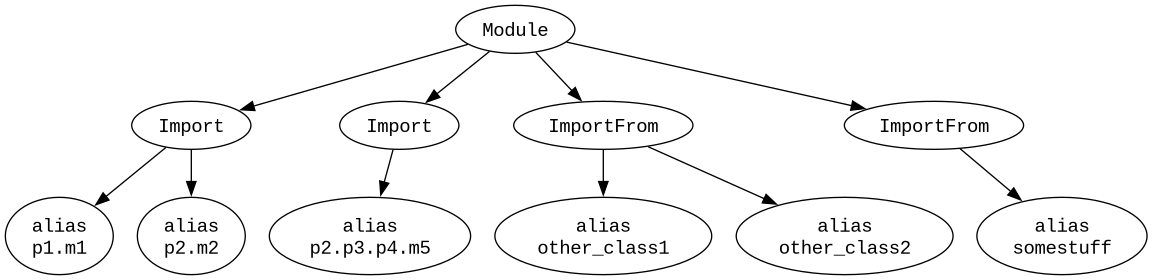
\includegraphics[width=0.5\textwidth]{assets/ast-example.png}
    \caption{Primjer AST-a}
    \label{fig:ast-example}
\end{figure}

\subsection{Tablice simbola}
Tablica simbola (eng.\ \textsl{symbol table}) je još jedna struktura podataka koju koriste kompajleri. Generira se nakon AST-a, te u Pythonovom slučaju direktno prethodi konačnoj kompilaciji. Kao i AST, moguć joj
je pristup kao objektu u Pythonu preko modula \texttt{symtable.py} (službena dokumentacija pod~\cite{docs:symtable}) iz standardne biblioteke. 

Tablica simbola sadrži sve simbole u kodu, a posebno se pritom osvrće na njihove opsege (\emph{scope}-ove) i eventualno neke dodatne atribute. Pritom, glavna tablica sadrži globalni nazivni prostor (\emph{namespace}), 
a može sadržavati i podtablice sa vlastitim, lokalnim nazivnim prostorima. U Pythonu, to je slučaj za nazivne prostore klasa i funkcija, ali ne, za razliku od drugih jezika, for-petlji ili sličnih blokova koje nemaju vlastiti 
nazivni prostor.

Budući da se tablica generira iz samog AST-a, sve što možemo napraviti s tablicama simbola možemo i sa samim AST-om. Ipak, uporaba modula iz standardne biblioteke smanjuje mogućnost greške i osigurava usklađenost s
Pythonovim kompajlerom. Za primjer toga što je sve dostupno u Pythonu, čitatelj može pogledati primjer ispisa u bilježnici
\begin{center}
\texttt{example/symtable_example.ipynb}
\end{center}
u repozitoriju projekta~\cite{repo}.



\newpage
\section{Konstrukcija grafa}
Apstraktno sintaksno stablo je i samo graf, ali se značajno razlikuje od grafa
kakvog smo opisali u~\ref{sec:uvod}. Primijetimo, još jednom, da
slijed vrhova i bridova u AST-u odgovara slijedu samog koda. Imena i atributi
definirani u njemu su smisleni Pythonovom interpreteru prilikom
dinamičkog izvođenja programa, ali da bismo sami mogli raspoznati imena,
njihove uloge i prodrijeti kroz ljudskom oku ponekad konvoluiranu strukturu AST-a,
potreban je dodatni rad. Zbog toga želimo AST transformirati u 
prikladniji oblik grafa, koji ćemo kasnije prenijeti u grafovsku bazu podataka, a
koja će omogućiti vizualizaciju grafa i izvršavanje upita.

Napomenimo da je izbor konkretne realizacije tog grafa, za koji smo dosad
dali samo inspiraciju, subjektivan. Implicitna shema grafa dana je u~\ref{subsec:implicitna}, 
no u ovom projektu uvijek nastojimo omogućiti jednostavno stvaranje varijanti na glavnu
izvedbu. Doista, za što je moguće temeljitije izvlačenje informacija
iz koda, potrebno je obratiti pažnju na veliki broj specijalnih slučajeva.
Specijalnih slučajeva ne samo da je puno, zbog čega će vjerojatno
uvijek biti novih ideja ili mišljenja, već njihovim uvođenjem
povećavamo kod i kompliciramo njegovu strukturu. Zato se u ovom
trenutku fokusiramo na osnovne funkcionalnosti sa što
elegantnijom strukturom.

Spomenutu transformaciju obavljamo u Pythonu, ali primijetimo
da je neke ideje moguće izvesti i unutar same baze. Kad je to moguće,
dobro je tako napraviti zbog boljih performansi i deklarativnog koda.

\subsection{Obrada jednog modula}
Započnimo s problemom analize jednog modula\footnote{u ovom kontekstu,
izraz \emph{modul} poistovjećujemo s \texttt{.py} datotekom},
 odnosno preslikavanja njegovog koda u graf kakav želimo. U tom problemu imamo
dva glavna cilja:
\begin{itemize}
\item \textit{Obilazak AST-a i izvlačenje informacija o imenima.} Prilikom obilaska AST-a, želimo trenutnom vrhu
dodati atribute (npr.\ tip ako je dan) i povući odgovarajuće bridove s nekim drugim vrhovima u grafu. U
preorder obilasku stabla, obilazimo sintaktičke elemente onim redom kojim su navedeni u kodu. Osim toga,
posebice za povlačenje bridova, potrebno nam je nekakvo praćenje konteksta, budući da u čistom
obilasku u svakom trenutku vidimo samo jedan vrh. U našoj implementaciji koristimo se strukturom
\texttt{SNode} koja osim podataka koje prenosimo u bazu, sprema i neke podatke važne za kontekst.
Pri obilasku koristimo razne \texttt{handler}-e, svaki od kojih je povezan sa specifičnom
vrstom ili vrstama vrha u AST-u. Na taj način enkapsuliramo željene funkcionalnosti unutar
jedne funkcije i dozvoljavamo fleksibilnost po pitanju njihovog izbora. Moguće je pri
obradi jednog vrha dodati njegovu djecu na stog za kasniju obradu, ali ih i ignorirati ili
obratiti odmah ako je to moguče ili prikladno.

\item \textit{Rezolucija imena.} Programski kod sastoji se od raznih imena, a njihovo značenje ovisi ne samo
o dinamičnom pridruživanju već i o nazivnom prostoru u kojemu se nalaze. Ključno je razlikovati dva
imena koja se nalaze u različitim prostorima (npr.\ svaka od dvije funkcije može imati vlastitu lokalnu
varijablu \texttt{x}), ali i prepoznati dva imena kao ista (posebice prilikom uvoza).
\end{itemize}

Ta dva cilja ispunjavamo pomoću tri obilaska:
\begin{enumerate}
\item \textit{Prvi obilazak.} U prvom obilasku prolazimo kroz tablicu simbola.
	Za svaki novi lokalni simbol dodajemo novi \texttt{SNode} i postavljamo
	kontekstualne veze --- roditelja i rječnik s vlastitom djecom kad simbol
	ima vlastiti nazivni prostor.
\item \textit{Drugi obilazak.} U drugom prolasku obilazimo AST i sve atribute dosad viđenih
	simbola dodajemo kao nove simbole.
\item \textit{Treći prolazak.} U trećem prolasku ponovo obilazimo AST. Fokusiramo se na ranije spomenute
	funkcionalnosti važne kod obilaska i uglavnom stvaramo bridove.
\end{enumerate}


\subsection{Proširenje na cijeli paket}
Da bismo analizirali cijeli paket\footnote{u ovom kontekstu, paket poistovjećujemo s
mapom (folderom); u prošlosti je mapa
morala imati \texttt{__init__.py} file da se smatra paketom, no u novijim verzijama
($\ge$3.3) nije obavezan}
koji se sastoji od većeg broja modula i potpaketa, potrebno je doraditi dosadašnji algoritam:
\begin{itemize}
\item Najprije je potreban još jedan "nulti" obilazak, ovaj put fileova u repozitoriju, kojim
nalazimo sve module i pakete (\texttt{__init__.py} može definirati uvoz i varijable na razini paketa)
koje moramo analizirati. I ovdje je bitno uspostaviti kontekstualne veze između paketa i modula.

\item Izvršavamo prvi obilazak svakog od modula\footnote{ovdje mislimo i na module i na pakete s
\texttt{__init__.py}-jem}
u proizvoljnom poretku.

\item U drugim obilascima, koje opet izvršavamo u proizvoljnom poretka, osim atributa analiziramo i
uvoz (\emph{import}) dodajući u graf relevantne bridove.
Ovo je bitno da bismo u trećem prolasku mogli uvezena imena ispravno povezati s vrhovima. Naime,
ako modul \texttt{X} uvozi iz \texttt{Y}, a \texttt{Y} iz \texttt{Z}, tada će prvo biti potrebno
uvesti simbole iz \texttt{Z} u \texttt{Y}, budući da \texttt{X} tranzitivno
uvozi i iz \texttt{Z}.

\item Treći obilazak izvršavamo kao ranije, ali u specifičnom poretku. Konkretno, nikad
ne počinjemo treći obilazak modula prije nego obiđemo one module iz kojih prvi uvozi.
To je moguće pod pretpostavkom da nema cirkularnosti u uvozu, što, iako nije
samo po sebi zabranjeno, može dovesti do nepredividivog ponašanja.

\end{itemize}



\newpage
\section{Baza}

\subsection{Implicitna shema} \label{subsec:implicitna}
U ovom potpoglavlju dajemo konkretnu implicitnu shemu naše grafovske baze,
uz ponovnu napomenu kako je uz modifikacije moguće postići razne varijacije na temu,
ovisno o osobnim izborima ili specijaliziranoj namjeni.

Sljedeće su prisutni tipovi (labele) vrhova: \texttt{Package},
\texttt{Module}, \texttt{Class}, \texttt{Function} i \texttt{Name}.
Glavno svojstvo svih vrhova je \texttt{fullname} koje predstavlja
puno ime objekta iz perspektive korijena paketa. Ono se razlikuje između
svaka dva različita vrha. Druga zajednička svojstva su \texttt{name},
\texttt{moduleName} i \texttt{packageName} koji su imena
bez prefiksa i olakšavaju neke vrste upita. Daljnja svojstva ovise o
tipu --- moduli, klase i funkcije mogu imati \texttt{docstring} (dokumentacijski string),
funkcije imaju svojstvo \texttt{isAsync} koje govori je li funkcija asinkrona, a
ostala imena mogu imati zabilježen tip (npr.\ \texttt{int} ili \texttt{str}).

Moguće je bilo dodati još tipova (npr.\ koji predstavljaju posebno metode,
atribute ili argumente) no to semantički prikazujemo bridovima na način koji ćemo opisati
u nastavku.

Sada navodimo tipove bridova:
\begin{itemize}
\item \texttt{WIHIN_SCOPE}. Govori da je prvi vrh definiran u nazivnom prostoru drugog. Implicitno, prvi vrh je ime, klasa ili funkcija,
dok je drugi paket, modul, klasa ili funkcija. Nadalje nećemo uvijek specificirati moguće tipove vrhova.

\item \texttt{ASSIGNED_TO_WITHIN}. Govori da je prvom vrhu pridružena vrijednost unutar opsega drugog.
\item \texttt{REFERENCED_WITHIN}. Govori da je prvi vrh "spomenut" unutar opsega drugog.

\item \texttt{IMPORTED_TO}. Govori da je prvi vrh uvezen u opseg drugog.
\item \texttt{IMPORTS_FROM}. Suprotno, drugi vrh uvezen je u opseg prvog. Ovaj brid nije uvijek
dualan prethodnom jer se odnosi isključivo na module i pakete.

\item \texttt{INHERITS_FROM}. Jedna klasa naslijeđuje drugu.

\item \texttt{METHOD}. Označava funkciju metodom klase.
\item \texttt{DECORATES}. Označava da je prvi vrh dekorator drugom.
\item \texttt{ARGUMENT}. Označava da je vrh argument u funkciji.

\item \texttt{ATTRIBUTE}. Označava da je vrh atributut drugog.

\item \texttt{RETURNS}. Govori da se vrh "spominje" u \texttt{return} naredbi funkcije. Ako postoji
logičko grananje ili drugi oblik kontrole toka programa, to se ignorira. Ovaj brid ne govori
što točno funkcija vraća, već samo ističe da postoji veza između vrha i vraćenog.
\item \texttt{ASSIGNED_TO}. Govori da se prvi vrh "spominje" u definiciji drugog. Ponovo,
kontrola toka ili višestruka pridruživanja se ignoriraju. Brid samo ističe da postoji veza,
a ne pokušava otpetljati kontrolu toka, dinamičko stanje ili smisao.

\item \texttt{TYPED_WITH}. Označava da je vrh tipiziran klasom. Ako nije tipiziran klasom
definiranom unutar paketa nego \emph{built-in} tipom, taj podatak se sprema kao svojstvo vrha.

\end{itemize}

U trenutnoj izvedbi bridovi najčešće nemaju svojstva, a iznimka je \texttt{alias} kod uvoza.

\newpage
\subsection{Aplikacija}
Funkcionalnosti paketa dostupne su preko CLI sučelja. Osnovnoj naredbi \texttt{pygdb}
možemo dodati argumente kojima određujemo URI servera baze, podatke za autentifikaciju
i ime baze. Ukoliko nisu dani, koriste se vrijednosti zadane unutar koda. 

Nakon toga, dostupne su tri podnaredbe (\textsl{subcommands}). Među njima je ključna
\texttt{add} kojom analiziramo paket i dobiveni graf šaljemo u bazu. Detaljnije
o tom problemu raspravljamo u~\ref{subsec:performanse}. Paket je
dan kao URI koji može biti lokacija na lokalnom računalu ili druga mapa 
dohvatljiva naredbom \texttt{git\- clone}. Drugi argumenti su stupanj \emph{logging}-a
i relativni put do početnog mjesta za analizu (često \texttt{src}).

Nakon što se paket prenese u bazu, upite je moguće vršiti unutar Neo4j Browser sučelja,
ali i pomoću podnaredbe
\texttt{query}. Rezultati upita vizualiziraju se pomoću Graphviz-a. Ta opcija
je potencijalno vrlo spora i nesigurna, dakle treba ju koristiti s oprezom
te eventualno ne izložiti korisnicima s nedovoljnim ovlastima ili za 
iste dodati funkcionalnosti koje bi onemogućile Cypher injection.

Treća podnaredba \texttt{clear} (alternativno \texttt{create}, \texttt{reset})
dozvoljava da se baza resetira, u smislu da se izbriše i stvori nova, a dodat će se
odabrana ograničenja i indeksi. Dodajemo ograničenje jedinstvenosti svojstva
\texttt{fullname}\footnote{vrhovi se upravo drže u rječniku u kojemu su \texttt{fullname} ključevi,
ali ovo ograničenje je svejedno korisno da spriječi korisnika da zabunom
unese isti paket dvaput; time se na \texttt{fullname} dodaje i indeks}, ograničenje
postojanja svojstva \texttt{name} kao i \emph{fulltext} indeks na istom
budući da očekujemo da će upravo to svojstvo često sudjelovati u upitima.

Za kraj potpoglavlja dajemo jedan primjer potpune naredbe: \\ \\
\texttt{
	python3 pygdb -{}-server bolt:\slash\slash localhost:7689\slash\ \textbackslash \\
	-{}-auth neo4j password -{}-database pygdb \textbackslash \\
	add -{}-uri git@github.com:pymc-devs\slash pymc -{}-relative pymc}

\subsection{Prijenos podataka i performanse} \label{subsec:performanse}
Najjednostavniji način za prijenos podataka iz internih
objekata u bazu je stvaranjem zasebne transakcije za svaki vrh
ili brid. Ta metoda ima dodatnu prednost jednostavnog i 
fleksibilnog koda, u smislu da istu funkciju možemo koristiti
za sve tipove vrhova ili bridova i za bilo kakvu konfiguraciju svojstava.
Drugim riječima, u ovoj metodi možemo unositi promjene
u postojeće tipove i svojstva bez da moramo imalo mijenjati kod
za prijenos u bazu. Velika mana ove metode je da je vrlo spora i to
naročito u stvaranju bridova --- njih je više i njihovo stvaranje
zahtijeva dva \texttt{MATCH}-a.

Alternativa je uporaba \emph{batch}-upita kako je preporučeno
i pokazano u~\cite{neo4j:performance}. Ova metoda doista znatno
skraćuje potrebno vrijeme i čini ga podnošljivim i za veće pakete.
Mana je u tome da, kao što je objašnjeno u~\cite{neo4j:params},
parametri ne mogu odgovarati labelama vrha ili tipu brida, nazivu
(ključu) svojstva niti su podržane parametarske mape kao u
prošlom slučaju. Zbog toga je tipove i atribute potrebno
hardkodirati, što komplicira stvaranje izmjena
u implicitnoj shemi.

Druga mogućnost za ostvarivanje boljih performansi je asinkroni driver.
Naravno, veću brzinu ne očekujemo u slučaju mnoštva jednostavnih
transakcija, već ga koristimo samo u \emph{batch} varijanti. Taj driver
je po navodu službene dokumentacije eksperimentalan, stoga postoji
i sinkrona verzija aplikacije u \texttt{sync_\-main.py}.

Razliku u performansama možemo prikazati na primjeru paketa
PyMC (kasnije u~\ref{subsec:pokazna}) s otprilike 66 tisuća bridova.
Dok kraj u prvoj varijanti nije bio ni na vidiku,
u drugoj je cjelokupni prijenos trajao 20 minuta.
Uvođenjem asikronog drivera, to se vrijeme gotovo pa prepolovilo.
\newpage

\newpage
\section{Primjeri}

\subsection{Pokazna baza} \label{subsec:pokazna}

\subsection{Primjeri upita} \label{subsec:primjer}

\subsection{Rezultati} \label{subsec:rezultati}

\newpage
\section{Osvrt}

\subsection{Nedostaci} \label{subsec:nedostaci}
Pythonova dinamičnost i fleksibilnost donose ozbiljne nedostatke ovakvom projektu od
početka. Navedimo tri značajna uzroka:

\begin{enumerate}

	\item \emph{Fleksibilnost u pridruživanju imena.} Kao što smo već spomenuli
u~\ref{subsec:python}, isto ime u toku programa može biti vezano za više
potpuno različitih objekata. Zbog toga, naši rezultati ne moraju u
svim slučajevima biti pouzdani, a mogu ispasti i zbunjujući. Ipak,
takvo recikliranje imena nije dobra praksa i ne očekujemo da ćemo ga
često viđati.

\item \emph{Dinamički generirani kod.} U Pythonu su mogući razni oblici koda
koje možemo smatrati dinamički generiranim. Takav kod je onda teško, ako
uopće moguće, analizirati unutar apstraktnog sintaksnog stabla.
Jedan primjer je Pythonova funkcija \texttt{exec} koja dan joj string
izvodi kao kod. Korištenje te funkcije je rijetkost i najčešće nije
dobra ideja.

Ipak, postoje drugi primjeri koji su puno češći. Primjer su
funkcije \texttt{getattr} i \texttt{setattr} koje upravljaju s
atributima objekta. Pritom se atribut daje kao string, a
ne mora biti \texttt{ast.Name} vrh već može biti rezultat
evaluacije nekog izraza ili iteratora.

Drugi važni primjer su funkcije iz standardne biblioteke
\texttt{importlib} koja omogućava veću kontrolu nad uvozom modula
i paketa. Ponovo, značenje njihovih argumenata može se skrivati
iza evaluacije kompliciranog i dinamički određenog izraza.
Uporaba biblioteke \texttt{importlib} upravo je češća u
sofisticiranijim paketima koji i zahtijevaju takve
dodatne funkcionalnosti. To predstavlja značajan problem unutar
ovog projekta jer ne možemo povezati imena uvezena na taj način
s objektima. Preostaje izbor --- stvarati duplikate za vrhove ili
ignorirati sva imena koja ne možemo rezolvirati. Duplicirani vrhovi
imaju memorijsku cijenu, a sama njihova prisutnost ne garantira
uvijek da će biti kao takvi prepoznati.

\item \emph{Objekti uvezeni iz koda u drugom jeziku.} U Pythonu
je moguće uvesti objekte i imena definirane u drugim 
programskim jezicima, a poznat su i česti slučaj C i
C++. Tada ni ta imena ne možemo rezolvirati bez značajnog
dodatnog napora. Znamenit primjer su Pythonovi \emph{built-in} moduli.
Primjerice, \texttt{ast.py}, koji je zapravo omotač,
uvozi modul \texttt{_ast.py} kreiran iz izvornog koda
u C-u (v.\ \cite{ast_u_c}).

\end{enumerate}

\subsection{Slični projekti} \label{subsec:slicni}

U trenutku pisanja rada, autor nije bio svjestan projekata
koji bi odgovarali ovom u funkcionalnostima, naime
izvlačenju semantičkih pojava u kodu u Pythonu, njihovom modeliranju
grafom i spremanju u grafovsku bazu podataka. Navedimo
dva projekta koji su donekle slični:

\begin{itemize}

\item \texttt{pyclrb.py} (v.\ \cite{docs:pyclbr}). Ovaj modul Pythonove
standardne biblioteke analizira klase i funkcije unutar jednog modula.
Za to se također koristi obilaskom AST-a.

\item \texttt{Pyan} (v.\ \cite{repo:pyan}). Ovaj paket, vjerojatno
najsličniji našem, statički analizira kod u jednoj ili više datoteka i
konstruira graf koji se može vizualizirati pomoću Graphviza. Također se
koristi AST-ovima i tablicama simbola. Osim razlika u implementaciji,
glavna je razlika da je konkretno riječ o statičkom \emph{call graph}-u,
dakle paket se bavi samo funkcijama, metodama, i njihovim međusobnim
pozivanjem.

\end{itemize}

Pored ovih paketa, postoji još obilje drugih koji s vlastitim, specifičnim,
namjenama vrše statičku analizu koda u Pythonu, pritom se
najčešće služeći sličnim alatima.




\newpage
\printbibliography

\end{document}

